\documentclass{beamer}

\usepackage[style=numeric,maxnames=2]{biblatex}
\usepackage{minted}
\usepackage{tikz}

\definecolor{lightgray}{gray}{0.9}
\definecolor{mediumslateblue}{HTML}{7B68EE}
\newcommand*\circled[1]{\tikz[baseline=(char.base)]{\node[shape=circle,fill,inner sep=2pt] (char) {\textcolor{white}{#1}};}} % chktex 36

\usepackage[orientation=portrait,size=a0,scale=1.1]{beamerposter}
\usetheme{JuelichPoster}
\setbeamertemplate{caption}[numbered] % number figures

\ExecuteBibliographyOptions{%
  sorting=nyt,
  bibwarn=true,
  isbn=false,
  url=true%
}
\addbibresource{references.bib}

\setbeamertemplate{partner1}{
\includegraphics{img/cscs}}
\setbeamertemplate{partner2}{
\includegraphics{HBP_logo.jpg}}

\begin{document}
\begin{frame}[t, fragile]
  \frametitle{
\includegraphics[width=0.66\linewidth]{img/arbor-lines-proto-colour-full}\\
  Hodgkin-Huxley Sensitivity Analysis with Arbor}
  \framesubtitle{Reproducing \citeauthor{TorresValderrama2015} \citeyear{TorresValderrama2015}: Uncertainty Propagation in Nerve Impulses Through \\
  the Action Potential Mechanism\\
  \tiny{Sebastian Schmitt (University of Göttingen), Nora Abi Akar, Ben Cumming, Stuart Yates (CSCS); \\
  Thorsten Hater, Brent Huisman, Anne Küsters (Forschungszentrum Jülich)}}
    
  \begin{columns}[onlytextwidth,T]
    \begin{column}{0.65\textwidth}
      We present a reimplementation of a study performed by \citeauthor{TorresValderrama2015} \cite{TorresValderrama2015},
      "Uncertainty Propagation in Nerve Impulses Through the Action Potential Mechanism".
      This study was conducted to establish the utility of Arbor and to be able to verify the results and claims of the original publication. In it, the sensitivity of the membrane voltage to variation in the parameters of the Hodgkin-Huxley model are investigated using the Sobol method.

    \end{column}
    \begin{column}{0.3\textwidth}
      \vspace*{-10ex}
      \begin{block}{Where to find us}
        \begin{description}
          \item[Website] \href{https://arbor-sim.org}{arbor-sim.org}
          \item[Source code] \href{https://github.com/arbor-sim/arbor}{github.com/arbor-sim/arbor}
          \item[Documentation] \href{https://docs.arbor-sim.org}{docs.arbor-sim.org}
          \item[Contact] \href{mailto:contact@arbor-sim.org}{contact@arbor-sim.org}
        \end{description}
      \end{block}
    \end{column}
  \end{columns}

  \vspace*{5ex}

  \begin{columns}[onlytextwidth,T]
    \begin{column}{0.36\textwidth}
      
      \begin{figure}[htp]
        \centering
        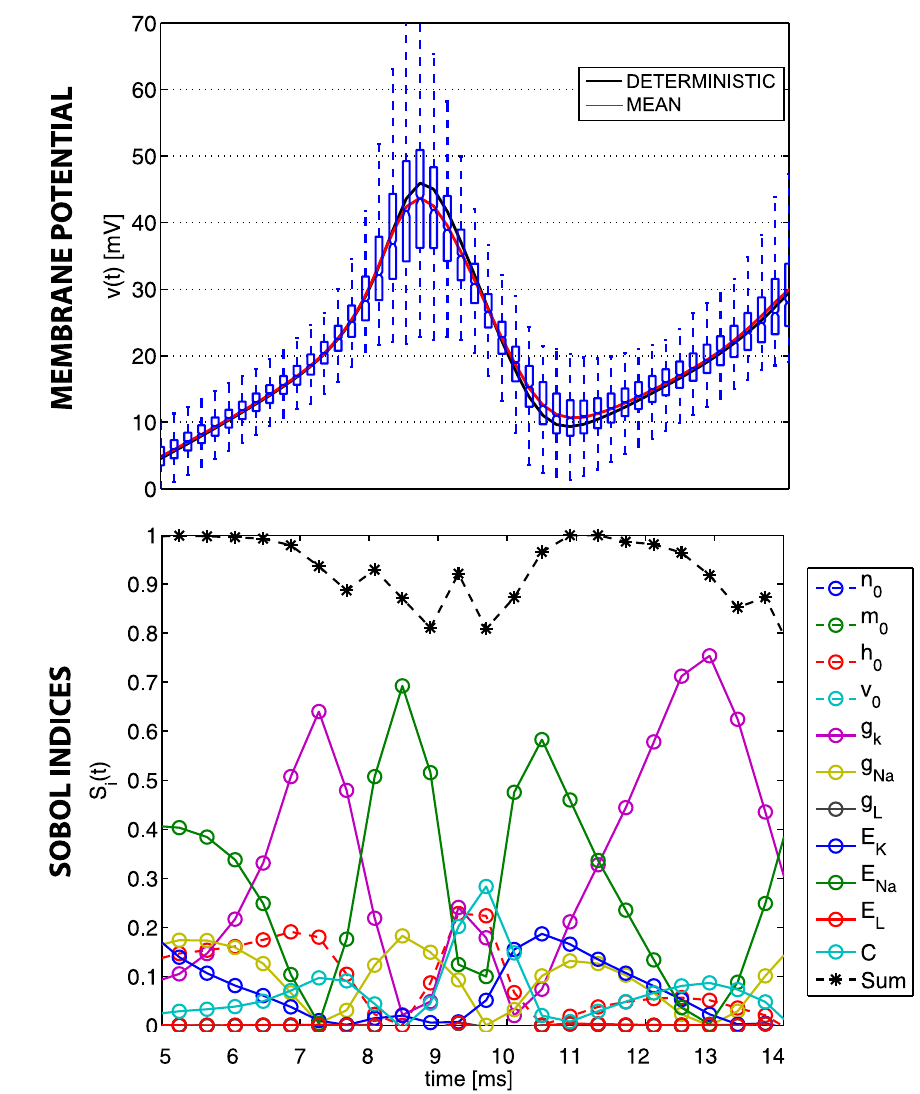
\includegraphics[width=\textwidth]{fig1a}
          \caption{Reproduced from figure 1a in \citeauthor{TorresValderrama2015} \citeyear{TorresValderrama2015}.
          Top: Membrane potential as function of simulation time. Bottom: the evolution of
          the individual Sobol indices and their sum. From this the conclusion is drawn that
          maximum conductance $\bar{g}_{K}$ and Nernst equilibrium potential $E_{Na}$ are
          together enough to estimate the variance of the original model to within 10\%
          difference for all time points.}
          \label{orig}
      \end{figure}

    \end{column}
    \begin{column}{0.63\textwidth}
      
      \begin{figure}[htp]
        \centering
        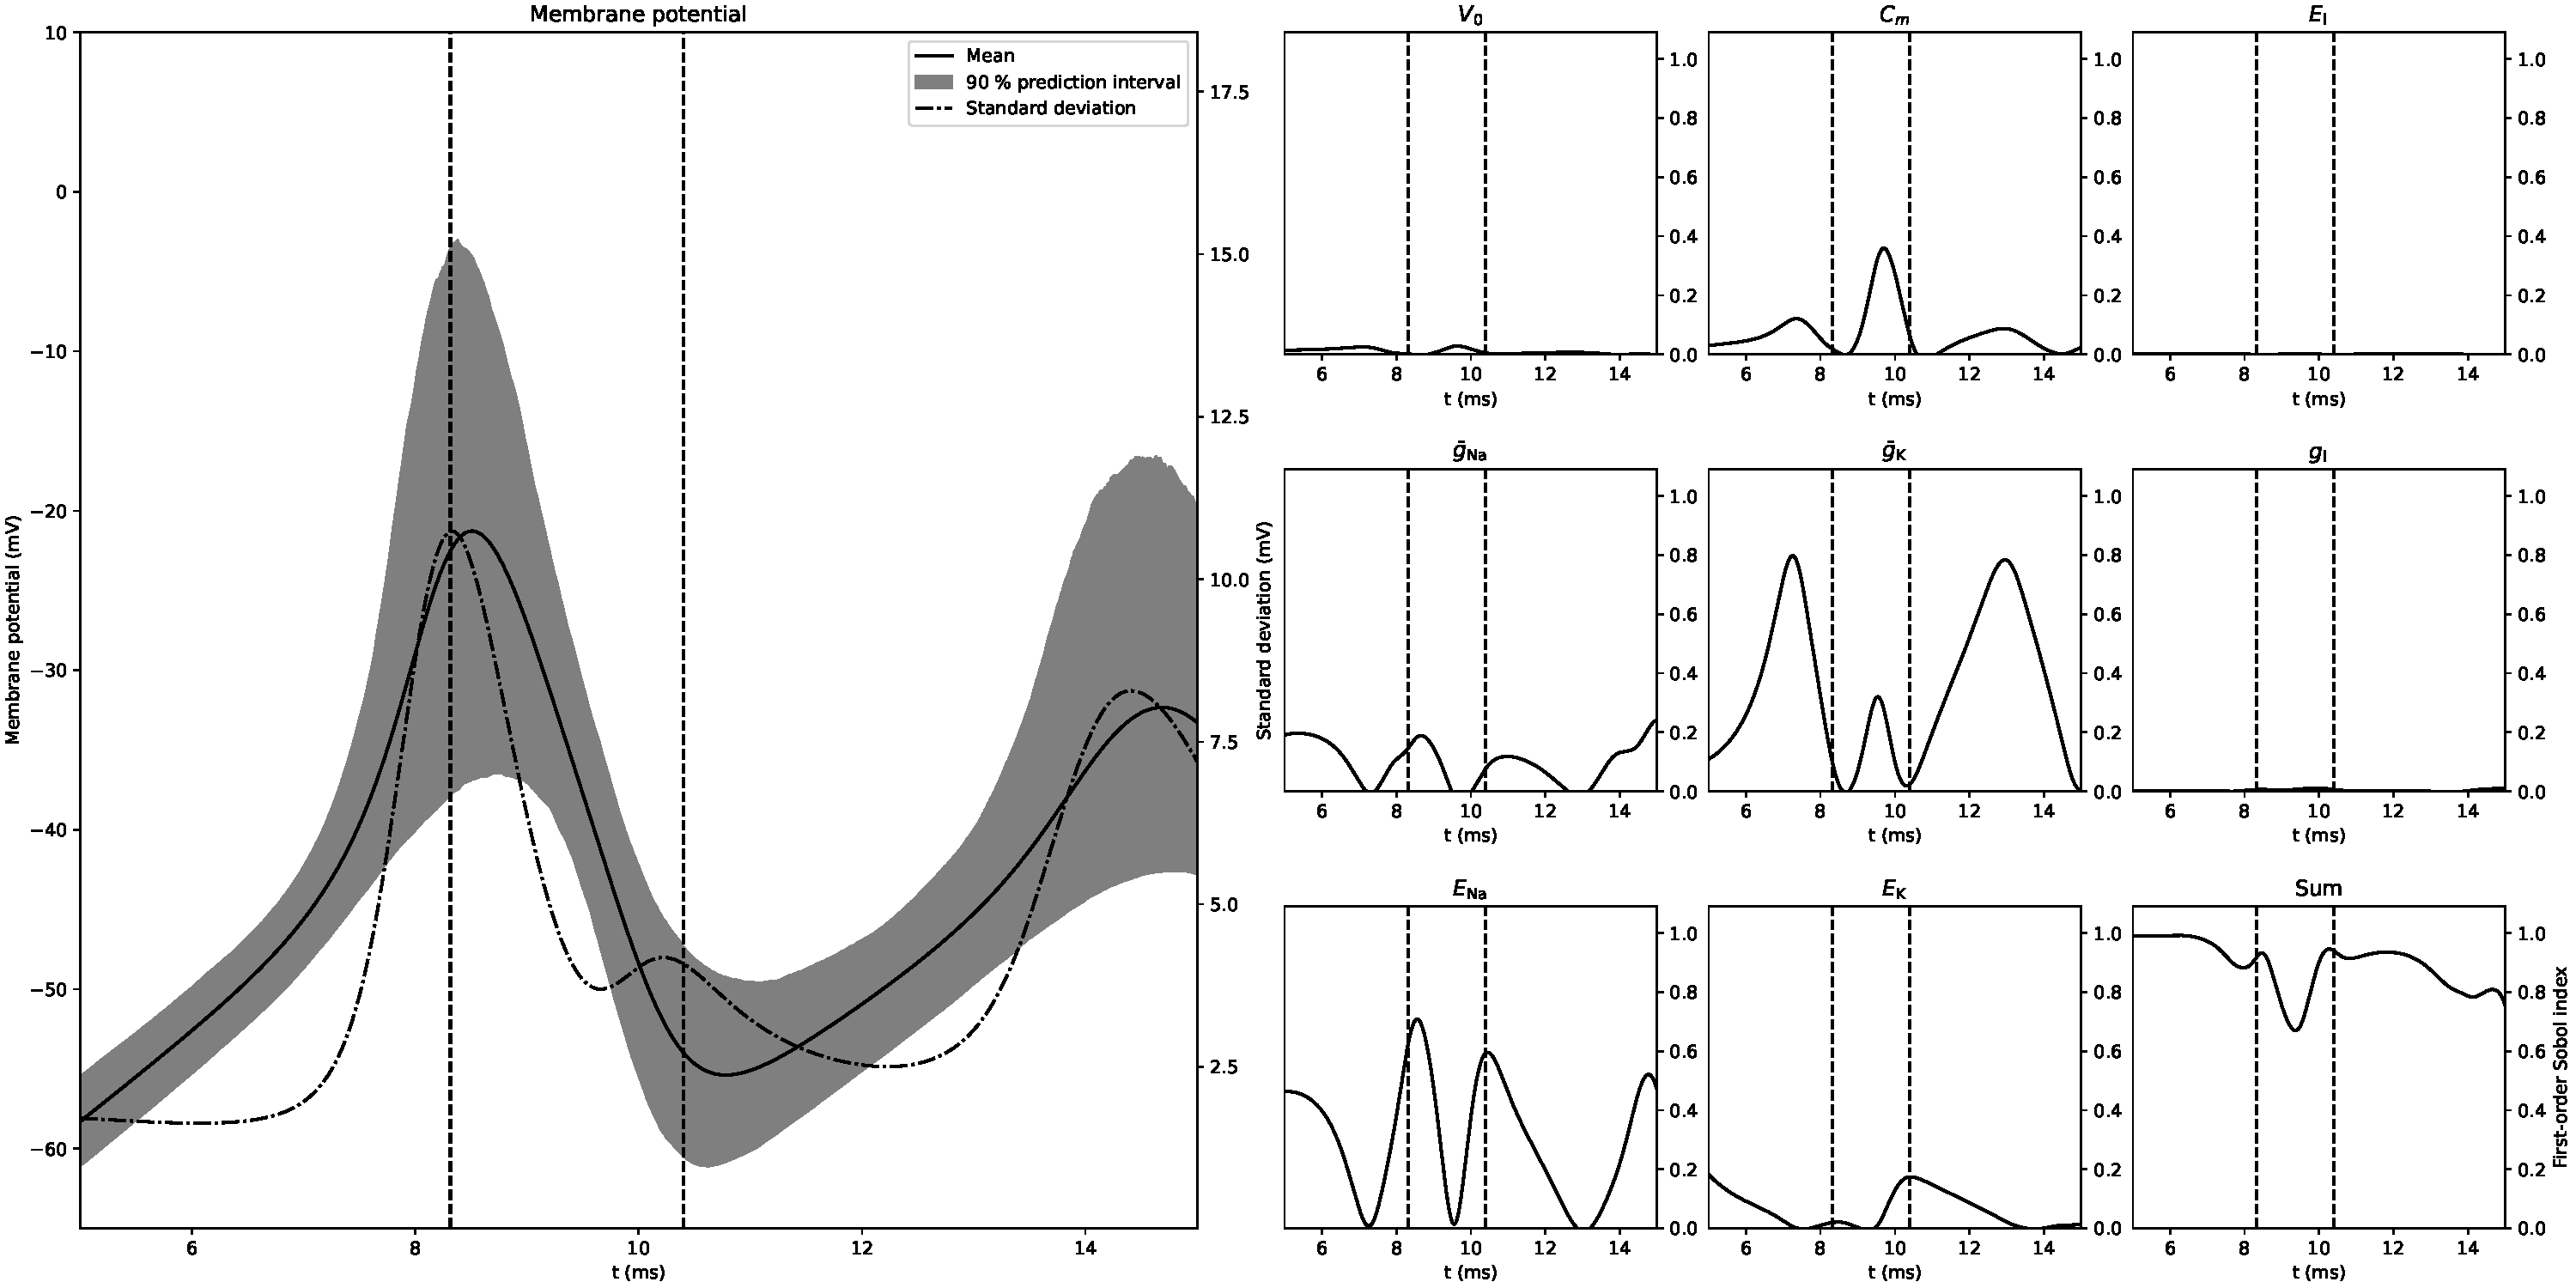
\includegraphics[width=\textwidth]{hh_sensitivity}
          \caption{Results reproduced for this poster.
          Left: Membrane potential as function of simulation time. Right: panels showing
          the evolution of the Sobol indices for the eight variables and their sum.
          as reproduced with Arbor and SALib.}
          \label{result}
      \end{figure}

    \end{column}
  \end{columns}

  \vspace*{-24ex}

  \begin{columns}[onlytextwidth]
    \begin{column}{.49\linewidth}
      \vspace*{24ex}

      \textbf{\structure{Abstract of \citeauthor{TorresValderrama2015} \citeyear{TorresValderrama2015}}}\\
      We investigate the propagation of probabilistic uncertainty through the action
      potential mechanism in nerve cells. Using the Hodgkin–Huxley (H-H) model
      and Stochastic Collocation on Sparse Grids, we obtain an accurate probabilistic
      interpretation of the deterministic dynamics of the transmembrane potential and gating
      variables. Using Sobol indices, out of the 11 uncertain parameters in the H-H model,
      we unravel two main uncertainty sources, which account for more than 90 \% of the
      fluctuations in neuronal responses, and have a direct biophysical interpretation. We
      discuss how this interesting feature of the H-H model allows one to reduce greatly the
      probabilistic degrees of freedom in uncertainty quantification analyses, saving CPU
      time in numerical simulations and opening possibilities for probabilistic generalisation
      of other deterministic models of great importance in physiology and mathematical neuroscience.

      We reproduce a plot of the main results in fig.~\ref{orig}.

      \vspace*{1ex}
      \textbf{\structure{Methods: Sobol Indices}}\\
      Variance-based sensitivity analysis (often referred to as the Sobol method
      or Sobol indices, after Ilya M. Sobol\cite{Sobol1993,Sobol2001}) is a form of global 
      sensitivity analysis. Working within a probabilistic framework, it decomposes 
      the variance of the output of the model or system into fractions which can
      be attributed to inputs or sets of inputs.

      From a black box perspective, any model may be viewed as a function $Y = f(X)$,
      where $X$ is a vector of d uncertain model inputs {$X_1$, $X_2$, ... $X_d$},
      and $Y$ is a chosen univariate model output.
      % A direct variance-based measure of sensitivity $S_i$, called the "first-order
      % sensitivity index", or "main effect index" is stated as follows:

      % \begin{equation}
      %   S_i = \frac{V_i}{Var(Y)}
      % \end{equation}

      % where
      
      % \begin{equation}
      %   \begin{aligned}
      %   Y & = f_0 + \sum_{i=1}^d f_i(X_i) + \sum_{i<j}^{d} f_{ij}(X_i,X_j) + \cdots + f_{1,2,\dots,d}(X_1,X_2,\dots,X_d)\\
      %   \operatorname{Var}(Y) & = \sum_{i=1}^d V_i + \sum_{i<j}^{d} V_{ij} + \cdots + V_{12 \dots d}\\
      %   V_{i} & = \operatorname{Var}_{X_i} \left( E_{\textbf{X}_{\sim i}} (Y \mid X_{i}) \right)\\
      %   V_{ij} & = \operatorname{Var}_{X_{ij}} \left( E_{\textbf{X}_{\sim ij}} \left( Y \mid X_i, X_j\right)\right) - \operatorname{V}_{i} - \operatorname{V}_{j}
      %   \end{aligned}
      % \end{equation}

      % This is the contribution to the output variance of the main effect of $X_i$,
      % therefore it measures the effect of varying $X_i$ alone, but averaged over
      % variations in other input parameters. It is standardised by the total variance
      % to provide a fractional contribution. Higher-order interaction indices $S_{ij}$,
      % $S_{ijk}$ and so on can be formed by dividing other terms in the variance
      % decomposition by $Var(Y)$.

      A direct variance-based measure of sensitivity $S_i$, called the "first-order
      sensitivity index", or "main effect index" is the contribution to the output variance of the main effect of $X_i$,
      therefore it measures the effect of varying $X_i$ alone, but averaged over
      variations in other input parameters. It is standardised by the total variance
      to provide a fractional contribution. Higher-order interaction indices $S_{ij}$,
      $S_{ijk}$ and so on can be formed by dividing other terms in the variance
      decomposition by $Var(Y)$. In the present study, we limit ourselves to first order
      indices.

      \vspace*{1ex}
      \textbf{\structure{Methods: Tools}}\\
      The two software components used in this replication are Arbor and SALib.

      Arbor \cite{Akar2019} simulates networks of spiking neurons,
      particularly multi-compartment neurons. In these networks, the 
      interaction between cells is conveyed by spikes and gap junction 
      and the multi-compartment neurons are characterized by axonal delays, 
      synaptic functions and cable trees. Each cell is modeled as a 
      branching, one-dimensional electrical system with dynamics derived 
      from the balance of transmembrane currents with axial currents that 
      travel through the intracellular medium, and with ion channels and 
      synapses represented by additional current sources.

      SALib \cite{Tennoe2018} is an open source library written in Python
      for performing sensitivity analyses. Instead, SALib is responsible for generating 
      the model inputs, using one of the sample functions, and computing 
      the sensitivity indices from the model outputs, using one of the 
      analyze functions.

    \end{column}
    \begin{column}{.49\linewidth}
      % \textbf{\structure{Methods: preparation}}\\

      % The parameters chosen are the same as in \citeauthor{TorresValderrama2015} \citeyear{TorresValderrama2015}, 
      % minus the intial conditions $n_0$, $m_0$, $h_0$:
      
      % \begin{equation}
      %   \xi = [ V_0, C_m E_{l}, \bar{g}_{Na}, \bar{g}_{K}, g_{l}, E_{Na}, E_{K} ]
      % \end{equation}

      % The parameter space of a 20\% variablity in the nominal values of the eight parameters is sampled 256 times using Saltelli’s\cite{Saltelli2004} extension of the Sobol’ sequence; \mintinline{Python}{SALib.sample.saltelli.sample()}.

      % % \begin{verbatim}
      % %   ./analysis.py --sample parameters_hh.npy
      % %   Sampling parameter space and saving to parameters_hh.npy
      % %   SALib.sample.saltelli.sample(problem, 2**8, calc_second_order=False)
      % % \end{verbatim}
      % % \cite{Saltelli2004}

      % \textbf{\structure{Methods: simulation}}\\
      % % Creating a simulation with Arbor follows four steps: 

      % % \begin{enumerate}
      % %   \item Define the full cell descriptions of all cells.
      % %   \item Define a recipe, which represents a set of neuron constructions 
      % %   and connections with mechanisms specifying ion channel and synapse 
      % %   dynamics in a cell-oriented manner. This has the advantage that 
      % %   cell data can be initiated in parallel.
      % %   \item Define the computational resources available to execute the model.
      % %   \item Initiate and execute a simulation of the recipe on the chosen hardware resources.
      % % \end{enumerate}
      % % Arbor makes a distinction between the description of a model, and
      % % the execution of a model: a recipe describes a model, and a simulation
      % % is an executable instantiation of a model.

      % The present study is about the parameters of the Hodgkin–Huxley model,
      % which in Arbor is a mechanism that can be 'painted' on (parts of) a cells
      % morphology. Since the morphology in this case is not relevant, a cylindric 
      % cell with diameter and length of 2 micrometer is created. The variables 
      % in formula eqn.~3 are parametrized and set for each simulation of the in the
      % previous step generated values.

      % % The recipe is similarly simple: there is a single cell and therefore
      % % no network. However, Arbor permit

      % % (((Simulations manage the instantiation of the model and the scheduling 
      % % of spike exchange as well as the integration for each cell group. 
      % % A cell group represents a collection of cells of the same type computed 
      % % together on the GPU or CPU. The partitioning into cell groups is provided 
      % % by a domain decomposition which describes the distribution of the model over 
      % % the locally available computational resources.)))

      \textbf{\structure{Method: Procedure}}\\
      A typical sensitivity analysis using SALib follows four steps:
      \begin{enumerate}
      \item Determine the model inputs (parameters) and their sample range.
      \item Run the sample function to generate the model inputs.
      \item Evaluate the model using the generated inputs, saving the model outputs.
      \item Run the analyze function on the outputs to compute the sensitivity indices.
      \end{enumerate}

      The parameters chosen are the same as in \citeauthor{TorresValderrama2015} \citeyear{TorresValderrama2015}, 
      minus the intial conditions $n_0$, $m_0$, $h_0$:
      
      \vspace*{-2ex}
      \begin{equation}
        \xi = [ V_0, C_m E_{l}, \bar{g}_{Na}, \bar{g}_{K}, g_{l}, E_{Na}, E_{K} ]
      \end{equation}

      The parameter space of a 20\% variablity in the nominal values of the eight parameters is sampled 256 times using Saltelli’s\cite{Saltelli2004} extension of the Sobol’ sequence; \mintinline{Python}{SALib.sample.saltelli.sample()}.

      The present study is about the parameters of the Hodgkin–Huxley model. in
      Arbor, Hodgkin–Huxley is a mechanism that is 'painted' on (parts of) a cells
      morphology. Since the morphology in this case is not relevant, a cylindric 
      cell with diameter and length of 2 $\mu m$ is created. The variables 
      in formula eqn.~1 are parametrized and set for each simulation of the in the
      previous step generated values. A current clamp of $140 \mu A/cm^2$ applied for 15
      ms. $m$, $n$, $h$ and the membrane voltage are probed every 10 $\mu s$ and stored to disk.

      Finally, a (first order) Sobol index is calculated for every timestep of every parameter, giving an indication of the relative contribution of each parameter;
      \mintinline{Python}{SALib.analyze.sobol.analyze()}.
      
      \vspace*{1ex}
      \textbf{\structure{Results and Conclusions}}\\
      
      The results are plotted in fig.~\ref{result}. Comparing the membrane potential
      and the Sobol indices with those in the original
      paper, excellent agreement is readily apparent. This strenghens the observations
      made in the original publication, as well as demonstrates the accuracy and 
      capability of Arbor for serious study in general, and the creation of a quick 
      toy simulation for verification of results.

      We have demonstrated how to setup and replicate a study using Arbor and SALib. Sources for the reproduction of the result are available at \cite{thisposter}.

      \vspace*{1ex}
      \textbf{\structure{References}}\\
      \renewcommand*{\bibfont}{\footnotesize}
      {\footnotesize \printbibliography{} }
      \vfill

      \textbf{\structure{Acknowledgements}}\\
      {\footnotesize This research has received funding from the European Union's Horizon 2020
      Framework Programme for Research and Innovation under the Specific Grant
      Agreements No.\,720270 (HBP SGA1), No.\,785907 (HBP SGA2), and No.\,945539
      (HBP SGA3).
      
      This study was conducted to establish the correctness and utility of Arbor as part of the "The Functional Interplay between Plasticity Processes on Arbor" (or FIPPA) collaboration between the Arbor development team and the group of Dr. Christian Tetzlaff in Göttingen. The goal of FIPPA is to extend the neural network simulator Arbor by key plasticity processes that will allow to simulate and analyze the long-term adaptive dynamics of large-scale, morphologically-detailed neuronal networks.}
    \end{column}
  \end{columns}

  
\end{frame}
\end{document}
